\documentclass[11pt,a4paper]{article}

% ==================== PAQUETES ====================
\usepackage[utf8]{inputenc}
\usepackage[T1]{fontenc}
\usepackage[spanish]{babel}
\usepackage{geometry}
\geometry{left=3cm, right=3cm, top=2.5cm, bottom=2.5cm}
\usepackage{setspace}
\usepackage{graphicx}
\usepackage{titlesec}
\usepackage{parskip}
\usepackage{helvet}
\renewcommand{\familydefault}{\sfdefault}
\usepackage{hyperref}
\usepackage{xurl}      % rompe URLs largas
\hypersetup{
    colorlinks=true,
    linkcolor=blue,
    urlcolor=blue,
    citecolor=blue
}
\usepackage{graphicx}
\usepackage{float}
\usepackage{microtype}
\usepackage{tikz}
\usepackage{xcolor}
\usepackage{tcolorbox}
\tcbuselibrary{skins}
\usepackage{fancyhdr}
\usepackage{enumitem}
\usepackage{amsmath}
\setlength{\abovedisplayskip}{5pt}
\setlength{\belowdisplayskip}{6pt}
\setlength{\abovedisplayshortskip}{4pt}
\setlength{\belowdisplayshortskip}{4pt}

% ==================== COLORES ====================
\definecolor{azuloscuro}{RGB}{10, 50, 100}
\definecolor{azulmedio}{RGB}{25, 65, 120}
\definecolor{dorado}{RGB}{180, 145, 60}
\definecolor{grisclaro}{RGB}{245, 245, 245}

% ==================== CONFIGURACIÓN ====================
\setstretch{1}
\pagestyle{fancy}
\fancyhf{}
\fancyfoot[C]{\thepage}   % Número centrado en el pie
\renewcommand{\headrulewidth}{0pt}

\titleformat{\section}
    {\normalfont\Large\bfseries\color{azuloscuro}}{\thesection.}{0.5em}{}
\titleformat{\subsection}
    {\normalfont\large\bfseries\color{azulmedio}}{\thesubsection.}{0.5em}{}

\titlespacing*{\section}
{0pt}{2.0ex plus 0.5ex minus 0.2ex}{1.0ex}

\titlespacing*{\subsection}
{0pt}{1.2ex plus 0.3ex minus 0.2ex}{0.5ex}

\begin{document}

% ==================== PORTADA ====================
\begin{titlepage}
% --- FONDO Y ELEMENTOS DECORATIVOS ---
\begin{tikzpicture}[remember picture, overlay]
    
    % 1. Barra lateral decorativa (se dibuja primero para quedar al fondo)
    \fill[azulmedio] (current page.north west) rectangle ([xshift=1.2cm]current page.south west);
    
    % 3. Línea dorada decorativa superior
    \fill[dorado] ([yshift=-6cm]current page.north west) rectangle ([yshift=-6.15cm]current page.north east);
    
    % 4. Caja inferior gris
    \fill[grisclaro] (current page.south west) rectangle ([yshift=3.9cm]current page.south east);
    
    % 5. Línea dorada decorativa inferior (para equilibrar el diseño)
    \fill[dorado] ([yshift=3.9cm]current page.south west) rectangle ([yshift=3.8cm]current page.south east);

        % 2. Fondo azul oscuro en la parte superior
    \fill[azuloscuro] (current page.north west) rectangle ([yshift=-6cm]current page.north east);
    \node[anchor=center] at ([xshift= 2.4 cm, yshift=-2.9 cm]current page.north west) {
\includegraphics[width=3.7cm]{complejo.png}};
    
    % --- TEXTOS ENCABEZADO Y PIE (Posicionamiento Absoluto) ---
    % Se ajusta xshift=0.6cm para centrar visualmente restando la barra lateral
    
    % Texto Superior (Institución)
    \node[anchor=center, text=white, align=center] at ([yshift=-3cm, xshift=1 cm]current page.north) {
        % \includegraphics[width=3cm]{logo.png} \\[0.3cm] % Descomenta si usas logo
        {\scshape\LARGE Complejo Educativo Thomas Jefferson}\\[0.3cm]
        {\scshape\large Infraestructura Tecnológica y Servicios Informáticos}
    };

    % Texto Inferior (Lugar y Fecha)
    \node[anchor=center, text=azuloscuro, align=center] at ([yshift=1.75cm, xshift=0.6cm]current page.south) {
        {\large\scshape Sonsonate, El Salvador}\\[0.15cm]
        {\large Junio 2026}\\[0.35cm]
    };
    
\end{tikzpicture}

% --- CONTENIDO CENTRAL DE LA PÁGINA ---

% Espacio para saltar el banner superior (6.15cm)
\vspace*{5cm}

\begin{center}
    \begin{tcolorbox}[
        enhanced,
        colback=white,
        colframe=azuloscuro,
        width=0.9\textwidth,
        arc=4mm,
        boxrule=1.5pt,
        drop shadow=azuloscuro!30!white, % Sombra suavizada e integrada
        borderline={0.5pt}{3pt}{dorado}, % ¡NUEVO! Detalle de borde interno dorado
        left=20pt,
        right=20pt,
        top=20pt,
        bottom=20pt
    ]
        \centering
        % ¡NUEVO! Líneas separadoras en dorado para mayor elegancia
        {\color{dorado}\rule{0.6\textwidth}{1pt}}\\[0.6cm]
        {\Huge\bfseries\color{azuloscuro} El impacto de la seguridad
        en el crecimiento económico\\[0.6cm]
        de El Salvador}\\[0.6cm]
        {\color{dorado}\rule{0.6\textwidth}{1pt}}\\[0.4cm]
        {\Large\itshape\color{azulmedio} Documento de investigación}
    \end{tcolorbox}
\end{center}



% --- INFORMACIÓN DE AUTORÍA ---
\begin{center}
    \vspace{1.5cm}
    {\large\bfseries\color{azuloscuro} Presentado por:}\\[0.30cm]
    {\Large Mario Alejandro Marroquín Meléndez}\\[0.8cm]

    {\large\bfseries\color{azuloscuro} Línea de investigación:}\\[0.15cm]
    {\large Economía del Desarrollo}
\end{center}

% Espacio inferior para evitar que el texto toque el banner gris
\vspace*{2.5cm}

\end{titlepage}
% 

\section*{Introducción}
\addcontentsline{toc}{section}{Introducción}

La relación entre seguridad, calidad institucional y desarrollo económico ha ocupado un lugar central dentro de la economía del desarrollo durante las últimas décadas. La literatura sobre economía institucional sostiene que el crecimiento económico depende, en gran medida, de la capacidad de las instituciones para garantizar el Estado de Derecho, proteger los derechos de propiedad y generar un entorno predecible para la inversión y la actividad productiva (North, 1990; Rodrik et al., 2004; Acemoglu \& Robinson, 2012). En este contexto, sociedades más seguras tienden a ofrecer mejores condiciones para la inversión, fortalecer el funcionamiento institucional y favorecer un crecimiento económico sostenido (World Bank, 2011).

Sin embargo, investigaciones más recientes plantean que la seguridad no constituye únicamente un determinante directo del desempeño económico, sino también una manifestación observable de la capacidad institucional de un Estado para hacer cumplir la ley, controlar la corrupción y mantener la estabilidad política (Kaufmann et al., 2010; World Bank, 2011). Desde esta perspectiva, la violencia no representa únicamente un problema de seguridad pública, sino un síntoma del funcionamiento de las instituciones encargadas de garantizar el orden jurídico y la gobernabilidad.

En consecuencia, la violencia puede entenderse como un indicador de debilidad institucional. Países con elevados niveles de criminalidad suelen presentar mayores dificultades para hacer cumplir la ley, menores niveles de confianza en las instituciones y un entorno menos favorable para la inversión y el desarrollo productivo (World Bank, 2011; UNODC, 2023). Asimismo, la evidencia internacional muestra que la calidad institucional constituye uno de los principales determinantes de las diferencias de desarrollo entre países, incluso por encima de factores geográficos o del grado de apertura comercial (Rodrik et al., 2004; Acemoglu \& Robinson, 2012). No obstante, la mayor parte de estos estudios analiza cambios graduales ocurridos durante largos períodos de tiempo, existiendo relativamente pocos casos contemporáneos donde las condiciones de seguridad hayan experimentado transformaciones abruptas.

El Salvador constituye uno de esos casos excepcionales. Entre 2015 y 2016 el país registró una de las tasas de homicidios más elevadas del mundo, superando los 100 homicidios por cada 100,000 habitantes. Posteriormente experimentó una reducción superior al 95 \% en menos de una década, pasando a ubicarse entre los países con menores niveles de homicidios de América Latina (UNODC, 2023; World Bank, 2024). La magnitud y velocidad de esta transformación convierten al país en un caso de especial interés para estudiar cómo responden las instituciones y la economía frente a un cambio abrupto en las condiciones de seguridad.

\begin{figure}[H]
    \centering
    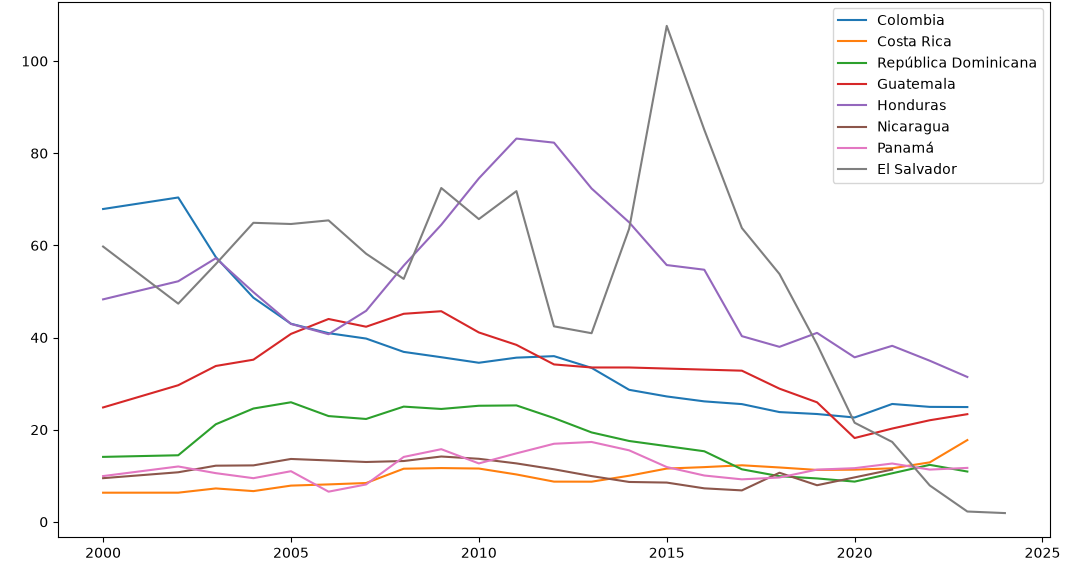
\includegraphics[width=0.73\textwidth]{homicide.png}
    \label{fig:homicidios}
\end{figure}

A partir de este contexto, la presente investigación busca responder la siguiente pregunta:

\begin{center}
\textit{¿Cómo se relacionan la seguridad, la calidad institucional y el desarrollo económico en Centroamérica, y qué revela el caso de El Salvador sobre dicho mecanismo de transmisión?}
\end{center}

La hipótesis central sostiene que la relación entre seguridad y crecimiento económico es predominantemente indirecta. En particular, se plantea que mayores niveles de violencia deterioran la calidad institucional ---especialmente el Estado de Derecho, el control de la corrupción y la estabilidad política---, reduciendo la capacidad de los países para atraer inversión extranjera y limitando, en consecuencia, su desempeño económico (North, 1990; World Bank, 2011; Acemoglu y Robinson, 2012).

Asimismo, se propone que estos efectos operan en diferentes horizontes temporales. Mientras las condiciones de seguridad pueden modificarse relativamente rápido como consecuencia de cambios en las políticas públicas, las instituciones evolucionan de manera más gradual y los efectos económicos requieren períodos aún mayores para reflejar plenamente dichas transformaciones. Bajo esta perspectiva, el crecimiento económico no respondería de forma inmediata a una reducción de la violencia, sino a través del fortalecimiento progresivo de las instituciones y de un entorno más favorable para la inversión.

La hipótesis central postula un mecanismo de transmisión en cuatro etapas:
\[
\underbrace{H_{it}}_{\text{Violencia}}
\;\xrightarrow{\;\beta_1 < 0\;}
\underbrace{Q_{it}}_{\text{Instituciones}}
\;\xrightarrow{\;\gamma_1 > 0\;}
\underbrace{F_{it}}_{\text{IED}}
\;\xrightarrow{\;\delta_1 > 0\;}
\underbrace{G_{it}}_{\text{Crecimiento PIB}}
\]
donde $H$ representa la tasa de homicidios, $Q$ la calidad institucional, $F$ la inversión extranjera directa y $G$ el crecimiento económico, $i$ indica el país y $t$ el año de la observación. Los signos sobre cada coeficiente indican la dirección esperada de las relaciones planteadas por la hipótesis de investigación.


\section*{Objetivos}
\addcontentsline{toc}{section}{Objetivos}

\subsection*{Objetivo general}

Analizar la relación entre la seguridad, la calidad institucional y el crecimiento económico en Centroamérica mediante un enfoque econométrico de datos de panel, complementado con técnicas de aprendizaje automático, con el propósito de identificar los mecanismos mediante los cuales la seguridad influye en el desempeño económico, tomando a El Salvador como estudio de referencia.
\subsection*{Objetivos específicos}

\begin{enumerate}
    \item Construir una base de datos de panel mediante la extracción, limpieza, integración y transformación de datos provenientes de organismos internacionales, garantizando la consistencia, comparabilidad y calidad de las variables económicas, institucionales y de seguridad utilizadas en el estudio.

    \item Diseñar e implementar un pipeline de análisis que integre técnicas matemáticas, econométricas y de aprendizaje automático para modelar las relaciones entre la seguridad, la calidad institucional y el crecimiento económico, incorporando procedimientos de validación, inferencia robusta y análisis de sensibilidad.

    \item Analizar e interpretar los resultados obtenidos mediante el pipeline, contrastándolos con la teoría de la economía institucional y la evidencia empírica disponible, con el fin de formular conclusiones sobre los mecanismos de transmisión y las diferentes velocidades de ajuste entre seguridad, instituciones y crecimiento económico.
\end{enumerate}

\section{Datos y metodología}

Para analizar esta hipótesis se construyó una base de datos de panel utilizando información proveniente de organismos internacionales de reconocido prestigio. Los indicadores económicos fueron obtenidos del \textit{World Development Indicators} (WDI) del Banco Mundial, los indicadores institucionales de los \textit{Worldwide Governance Indicators} (WGI) y las estadísticas de homicidios de la \textit{United Nations Office on Drugs and Crime} (UNODC).

La base de datos integra información anual para ocho países de Centroamérica y República Dominicana durante el período 2000--2024, generando un panel de aproximadamente 180 observaciones país-año. El proceso de construcción comprendió un flujo completo de extracción, transformación y carga (ETL), incluyendo la armonización de unidades de medida entre fuentes, tratamiento de valores faltantes, validación de consistencia temporal, generación de variables derivadas y verificación de la estructura del panel antes del análisis econométrico, el dataset, código, documentación y gráficos adicionales se encuentran en:
\begin{center}
\url{https://github.com/mariomarroquin3/data_analyzer}
\end{center}

Las principales variables incluidas fueron:

\begin{itemize}
\item Tasa de homicidios por cada 100\,000 habitantes.
\item Crecimiento anual del PIB.
\item Inversión extranjera directa como porcentaje del PIB.
\item Exportaciones como porcentaje del PIB.
\item Inflación.
\item Desempleo.
\item PIB per cápita (transformado mediante logaritmo natural).
\item Población (transformada mediante logaritmo natural).
\item Llegadas internacionales de turistas (transformadas mediante logaritmo natural).
\item Estado de Derecho (Rule of Law).
\item Control de la Corrupción (Control of Corruption).
\item Estabilidad Política (Political Stability).
\end{itemize}

Dado que los tres indicadores institucionales presentan una elevada correlación y describen dimensiones complementarias de un mismo fenómeno, se construyó un Índice Institucional mediante Análisis de Componentes Principales (Principal Component Analysis, PCA). Previamente, cada indicador fue estandarizado mediante puntuaciones $z$, garantizando que todos contribuyeran en igualdad de condiciones al índice sintético. El primer componente principal explicó aproximadamente el $78.9\%$ de la variabilidad conjunta y el índice alcanzó un Alfa de Cronbach de $\alpha=0.863$, indicando una elevada consistencia interna entre las dimensiones institucionales consideradas.

Con el fin de explorar la estructura de correlación entre las variables utilizadas en el análisis, se realizó un análisis exploratorio previo.

\begin{figure}[h]
\centering
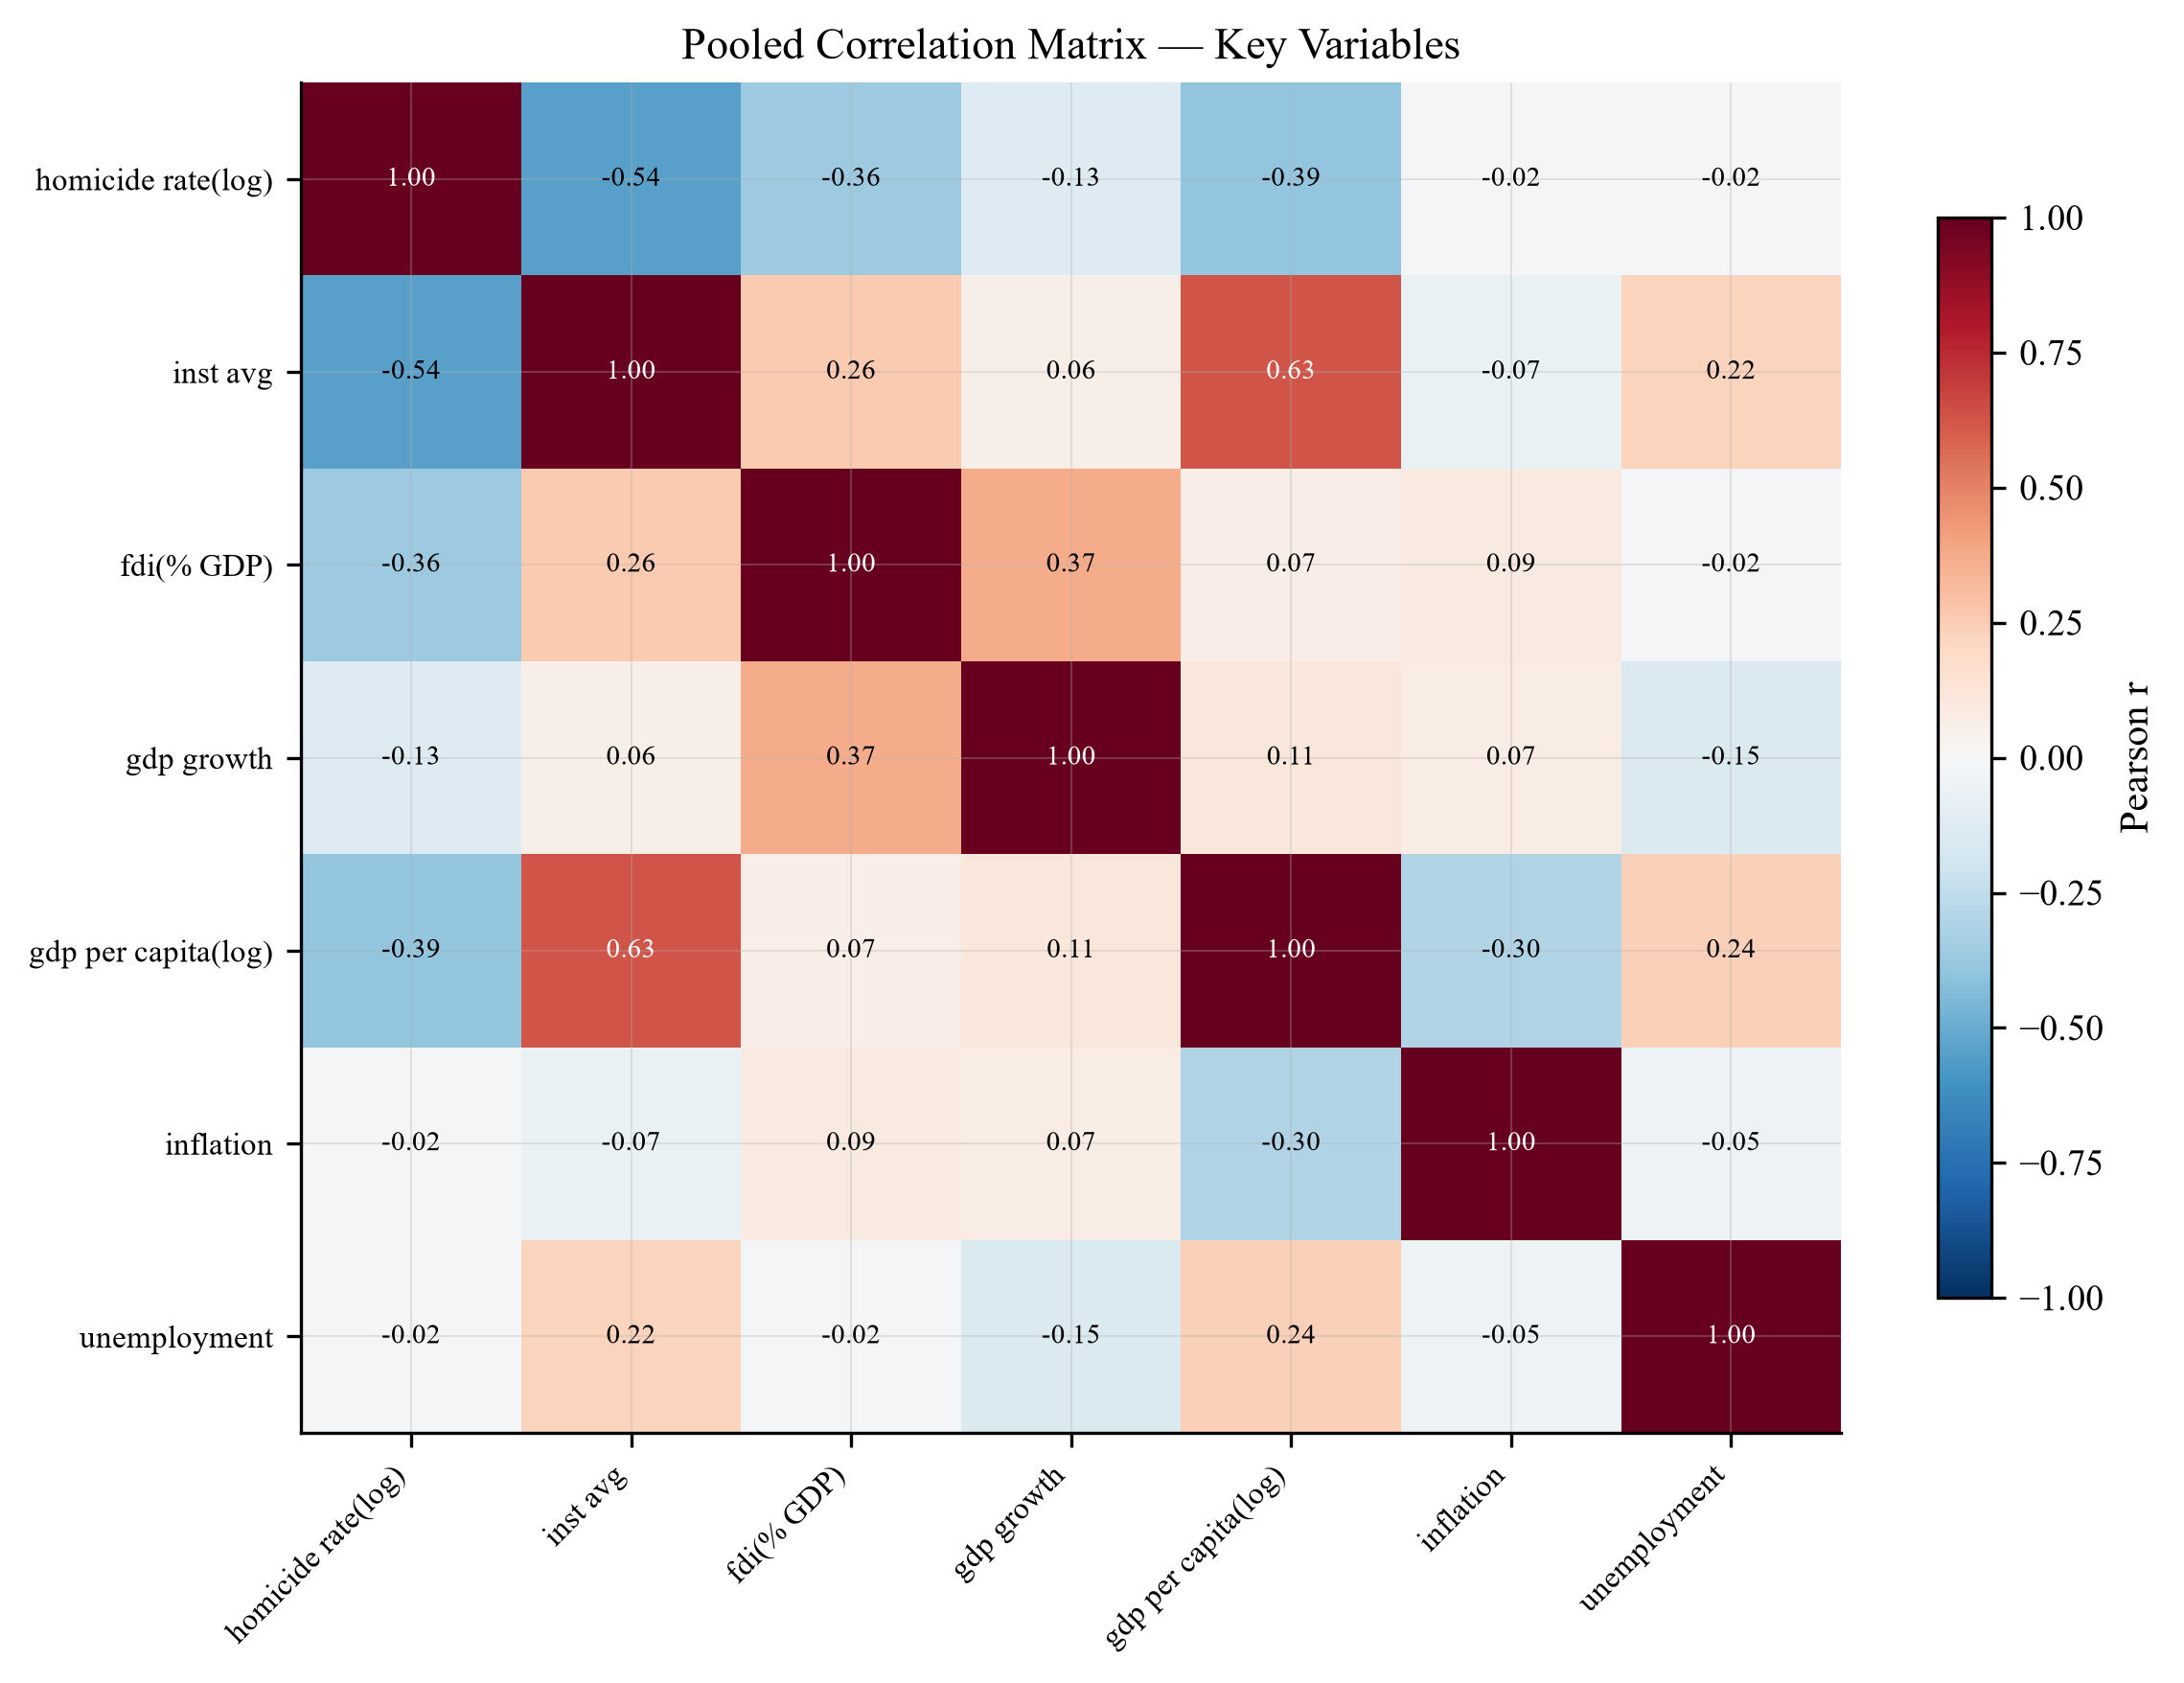
\includegraphics[width=0.85\textwidth]{03_correlation_heatmap.png}
\caption{Matriz de correlación entre variables de seguridad, instituciones y crecimiento económico.}
\label{fig:corr_heatmap}
\end{figure}

El análisis estadístico se desarrolló de manera secuencial. Inicialmente se realizaron análisis descriptivos mediante estadísticas resumen, matrices de correlación y visualizaciones exploratorias. Posteriormente se estimaron modelos de regresión lineal múltiple (OLS) como referencia metodológica. Finalmente, las relaciones principales fueron evaluadas mediante modelos de datos de panel con efectos fijos bidireccionales (\textit{Two-Way Fixed Effects}), incorporando efectos específicos por país y por año para controlar tanto la heterogeneidad no observada entre países como los choques comunes que afectan simultáneamente a toda la región.

Considerando que el panel está compuesto únicamente por ocho países, la inferencia estadística se fortaleció mediante errores estándar de Driscoll--Kraay, robustos frente a heterocedasticidad, autocorrelación serial y dependencia transversal, así como mediante procedimientos de Wild Cluster Bootstrap, recomendados para paneles con pocos clústeres. La estabilidad de las estimaciones fue además evaluada mediante análisis \textit{Leave-One-Country-Out} (LOCO), verificando que los resultados principales permanecieran consistentes al excluir individualmente cada país de la muestra.

Como complemento al análisis econométrico se implementaron modelos de aprendizaje automático basados en Random Forest Regressor y Gradient Boosting Regressor. Estos modelos no fueron utilizados para establecer relaciones causales, sino para evaluar la importancia relativa de las variables explicativas, detectar posibles relaciones no lineales y contrastar la consistencia de los resultados obtenidos mediante los modelos econométricos tradicionales.

\subsection{Evidencia regional}

El análisis descriptivo muestra que la violencia mantiene una relación estrecha con la calidad institucional de los países analizados. En términos generales, aquellos países que presentan mayores tasas de homicidios también exhiben menores niveles de Estado de Derecho, control de la corrupción y estabilidad política, resultado consistente con la literatura sobre economía institucional.

\begin{figure}[h]
\centering
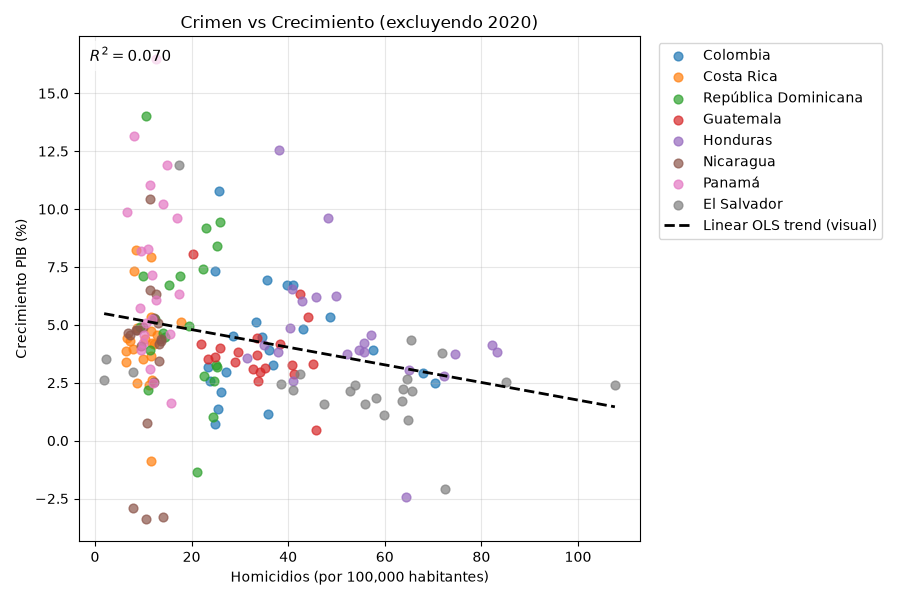
\includegraphics[width=0.79\textwidth]{Figure_2.png}
\caption{Relación entre homicidios y crecimiento económico (excluyendo 2020 por shock exógeno COVID-19).}
\label{fig:crime_growth}
\end{figure}

En contraste, la asociación bivariada entre la violencia y el crecimiento económico resulta débil y heterogénea entre países. El bajo poder explicativo del modelo lineal simple ($R^2 \approx 0.07$) sugiere que la relación entre ambas variables no es directa ni estable, sino que está fuertemente condicionada por la heterogeneidad institucional y por mecanismos de transmisión intermedios.

Esta evidencia preliminar respalda la hipótesis central del estudio, según la cual la seguridad no afecta al crecimiento de manera inmediata, sino a través de su impacto sobre la calidad institucional y, posteriormente, sobre la inversión y la acumulación de capital. En este sentido, la ausencia de una relación lineal fuerte no invalida el vínculo teórico, sino que refuerza la necesidad de un enfoque estructural y dinámico del proceso de desarrollo económico.

\subsection{Resultados econométricos principales}

Los modelos de efectos fijos bidireccionales estimados en el pipeline confirman este mecanismo de transmisión en tres etapas:

\textbf{Ecuación 1 (Violencia $\rightarrow$ Instituciones):}

La tasa de homicidios presenta un efecto negativo sobre el índice institucional:

\[
\beta = -0.1404, \quad p = 0.303
\]

El signo es consistente con la teoría institucional, aunque la significancia estadística disminuye bajo inferencia robusta (Driscoll--Kraay y clustering por país).

\textbf{Ecuación 2 (Instituciones $\rightarrow$ Inversión):}

La calidad institucional tiene un efecto positivo sobre la inversión extranjera directa:

\[
\beta = 0.9000, \quad p = 0.055
\]

Este resultado es marginalmente significativo bajo errores clusterizados y se mantiene estable en especificaciones alternativas del modelo.

\textbf{Ecuación 3 (Inversión + Instituciones $\rightarrow$ Crecimiento):}

La inversión extranjera presenta una asociación positiva con el crecimiento económico:

\[
\beta = 0.1371, \quad p = 0.213
\]

El efecto directo de las instituciones sobre el crecimiento pierde significancia cuando se incluye la inversión, lo que sugiere un mecanismo de mediación parcial.

\subsection{Interpretación estructural del sistema}

En conjunto, los resultados permiten proponer la siguiente cadena de transmisión:
\vspace{-0.25em}
\[
\text{Violencia}
\longrightarrow
\text{Calidad Institucional}
\longrightarrow
\text{Inversión Extranjera Directa}
\longrightarrow
\text{Crecimiento Económico}
\]

Sin embargo, el resultado más importante del pipeline no es únicamente la magnitud de los coeficientes, sino la \textbf{estructura temporal del ajuste económico}.

El alcance temporal de los datos y resultados sugiere que estos procesos no ocurren simultáneamente:

El interés de este marco no radica únicamente en la magnitud de los coeficientes estimados, sino en la interpretación dinámica del sistema. Los distintos componentes del modelo operan en horizontes temporales heterogéneos: la violencia puede ajustarse rápidamente ante cambios en política pública, mientras que las instituciones evolucionan de manera gradual debido a su naturaleza acumulativa. Finalmente, el crecimiento económico refleja estos cambios con mayor rezago, a medida que los agentes económicos ajustan decisiones de inversión y producción.

Es importante señalar que esta relación no debe interpretarse como estrictamente unidireccional. En la literatura de economía política e instituciones se ha documentado la existencia de endogeneidad bidireccional entre violencia e instituciones, en la medida en que instituciones débiles pueden facilitar mayores niveles de criminalidad, mientras que altos niveles de violencia también erosionan la capacidad institucional del Estado (Besley and Persson, 2011). Este problema de simultaneidad refuerza la necesidad de utilizar enfoques de datos de panel con efectos fijos y errores estándar robustos, ya que la estimación mediante modelos bivariados simples podría subestimar la complejidad del mecanismo de interacción entre ambas variables.

\subsection{Consistencia metodológica del pipeline}

Los resultados son robustos bajo múltiples enfoques:

\begin{itemize}
\item Efectos fijos bidireccionales (país y tiempo).
\item Errores estándar Driscoll--Kraay.
\item Clustering por país (G = 8).
\item Wild Cluster Bootstrap (inferencia principal).
\item Leave-One-Country-Out (robustez estructural).
\item Modelos de machine learning (Random Forest / Gradient Boosting).
\end{itemize}

En particular, los modelos de aprendizaje automático confirman que las variables institucionales y de violencia se encuentran entre los predictores más importantes del crecimiento económico, aunque sin implicar relaciones lineales estrictas.

En conjunto, el sistema de ecuaciones estimado presenta coherencia en los signos teóricos esperados, aunque con distinta intensidad estadística según la etapa del mecanismo.

\subsection{Validación cruzada Leave-One-Country-Out (LOCO-CV)}

Con el fin de evaluar la estabilidad estructural de las relaciones estimadas, se implementó un procedimiento de validación cruzada tipo Leave-One-Country-Out (LOCO-CV), en el cual cada país es excluido secuencialmente del conjunto de entrenamiento y utilizado como conjunto de prueba. Este enfoque permite analizar la robustez de los modelos ante heterogeneidad transversal y posibles dependencias específicas por país.

\begin{figure}[H]
    \centering
    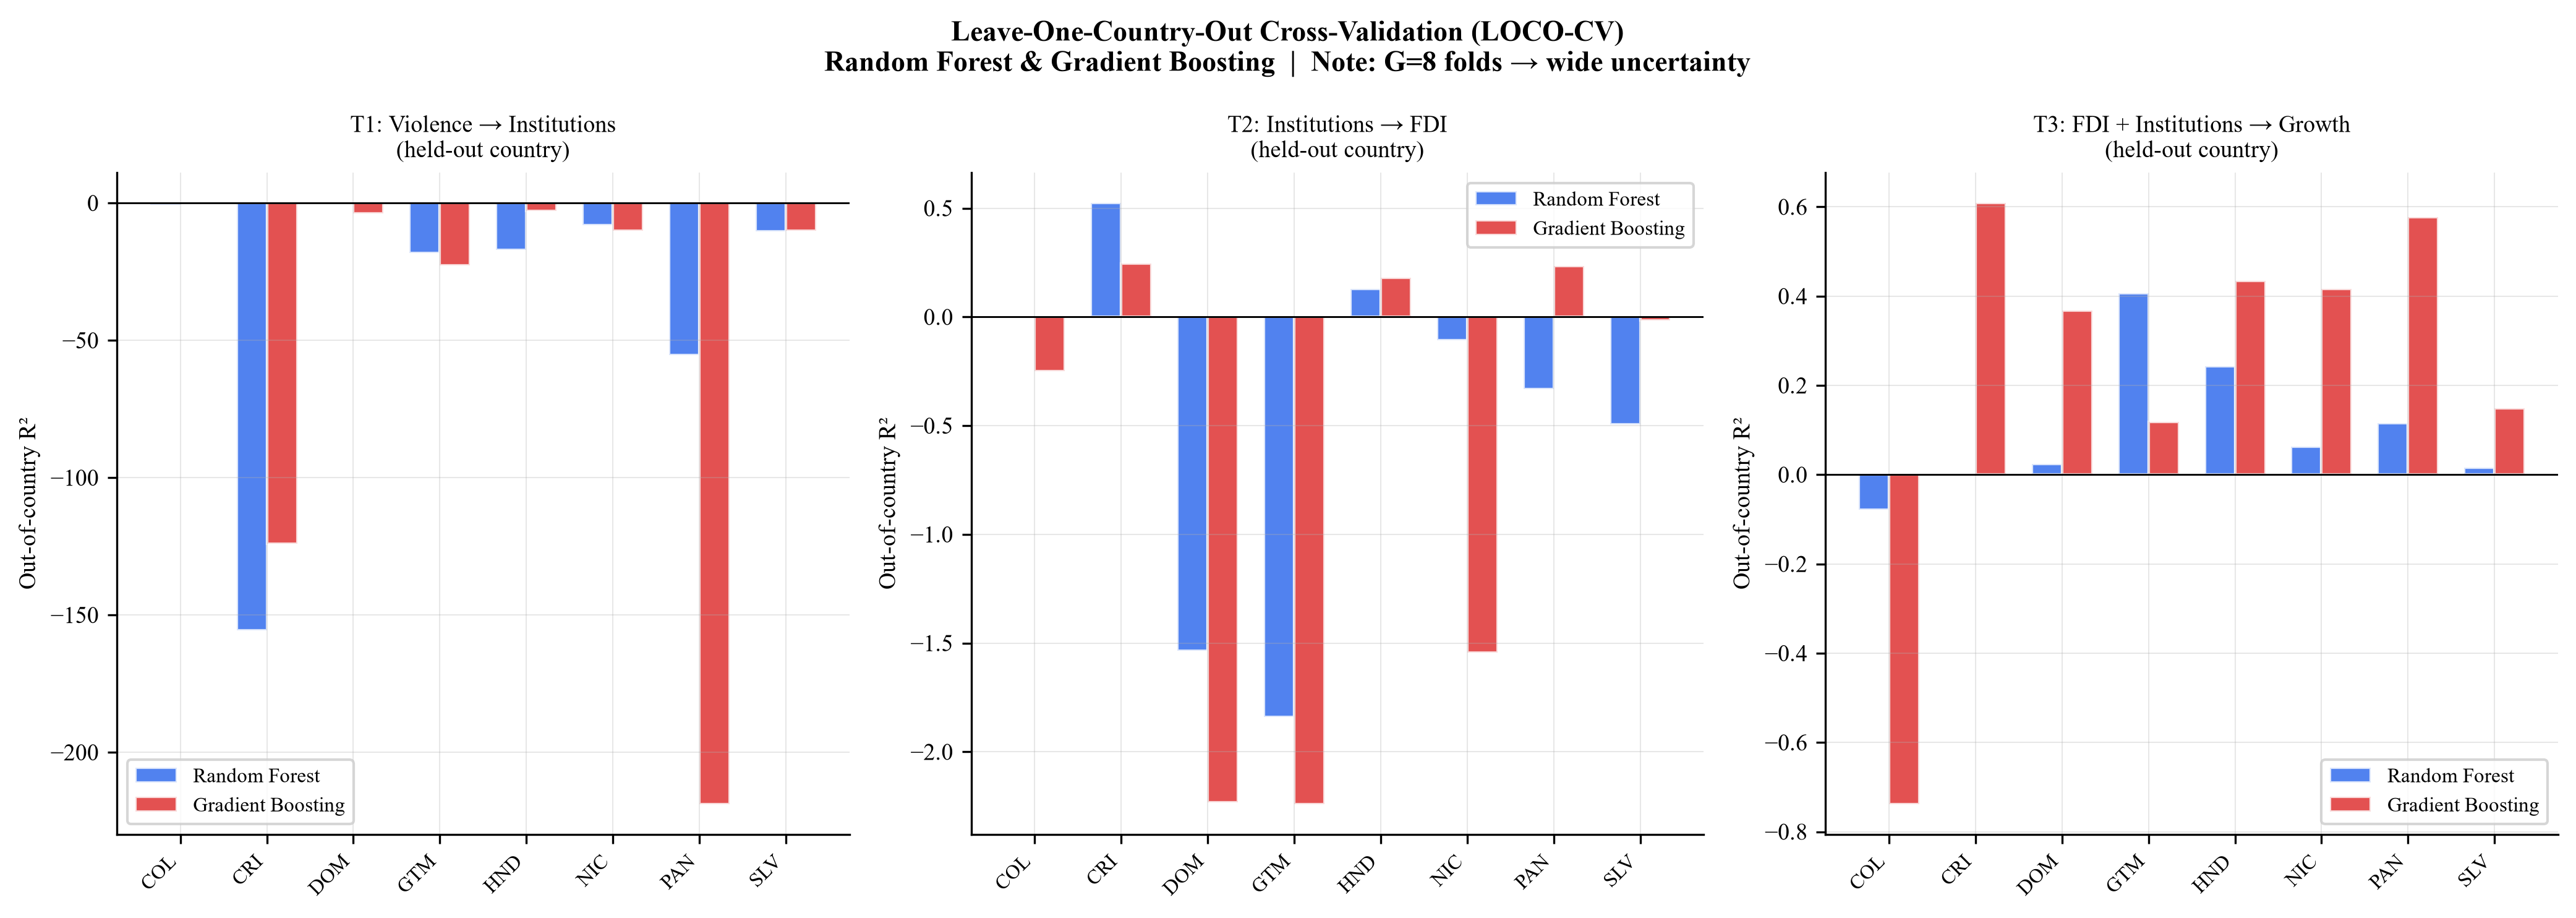
\includegraphics[width=0.95\textwidth]{08_ml_loco_cv.png}
    \caption{Validación cruzada Leave-One-Country-Out (LOCO-CV) para tres relaciones del sistema: (T1) violencia e instituciones, (T2) instituciones e inversión extranjera directa, y (T3) inversión e instituciones sobre crecimiento económico. Se comparan modelos Random Forest y Gradient Boosting.}
    \label{fig:loco_cv}
\end{figure}
\vspace{-1em}
Los resultados muestran una elevada heterogeneidad en la capacidad predictiva de los modelos a través de los distintos países. En la relación entre violencia e instituciones (T1), los valores de $R^2$ fuera de muestra son en su mayoría negativos o cercanos a cero, lo que indica una débil capacidad de generalización y una relación estructural inestable entre ambas variables.

De forma similar, la relación entre instituciones e inversión extranjera directa (T2) presenta una alta variabilidad entre países y signos inconsistentes en el desempeño predictivo, lo que sugiere que este vínculo no es homogéneo en la región y depende de características idiosincráticas de cada economía.

En contraste, el modelo que incorpora simultáneamente inversión e instituciones para explicar el crecimiento económico (T3) presenta un desempeño consistentemente superior, especialmente bajo Gradient Boosting, con valores positivos de $R^2$ en la mayoría de los países excluidos. Este resultado sugiere que el crecimiento económico responde mejor a la interacción conjunta de variables institucionales y de inversión, más que a relaciones bivariadas simples.

En conjunto, la evidencia obtenida mediante LOCO-CV refuerza la hipótesis de que el proceso de desarrollo económico opera a través de mecanismos no lineales y con fuertes efectos de heterogeneidad entre países.
\section*{Conclusiones}
\addcontentsline{toc}{section}{Conclusiones}

Los resultados muestran que la reducción de la violencia, por sí sola, no se traduce necesariamente en un incremento inmediato del crecimiento económico. Aunque las estimaciones mantienen los signos esperados por la teoría institucional, la evidencia sugiere que la relación entre seguridad y crecimiento opera principalmente de forma indirecta. En particular, el bajo poder explicativo del modelo bivariado entre homicidios y crecimiento ($R^2 \approx 0.07$) refuerza la ausencia de una relación contemporánea estable.

El principal aporte de esta investigación consiste en proponer un marco interpretativo dinámico en el que la seguridad, las instituciones y el crecimiento no evolucionan de manera simultánea, sino que conforman un sistema con rezagos heterogéneos. En este sistema, las condiciones de seguridad pueden modificarse relativamente rápido mediante políticas públicas, mientras que las instituciones responden a procesos acumulativos de largo plazo asociados al fortalecimiento del Estado de Derecho, la estabilidad política y el control de la corrupción. Finalmente, las variables macroeconómicas incorporan estos cambios de manera gradual, conforme los agentes económicos ajustan sus decisiones de inversión y producción.

Desde esta perspectiva, la ausencia de una relación contemporánea fuerte entre violencia y crecimiento económico no contradice la teoría institucional, sino que es consistente con un proceso de transmisión con rezagos, en el que los efectos económicos aparecen de forma diferida debido a la distinta velocidad de ajuste de cada dimensión del sistema.

En conjunto, la evidencia obtenida permite interpretar la seguridad no únicamente como un determinante aislado del crecimiento, sino como una manifestación observable de la capacidad institucional del Estado. En este sentido, una reducción sostenida de la violencia refleja la consolidación del monopolio de la fuerza y la disminución de los costos de transacción y de cumplimiento que enfrentan los agentes económicos. Sin embargo, estos efectos no se materializan de forma inmediata en los agregados macroeconómicos, sino que operan a través de ajustes progresivos en la estructura productiva.

El caso de El Salvador ilustra claramente esta dinámica asincrónica. La rápida reducción de la criminalidad constituye un cambio estructural en las condiciones de seguridad; sin embargo, sus efectos iniciales tienden a manifestarse a nivel microeconómico, mediante reducciones en costos operativos del tejido empresarial existente y del sector informal, que conforma, alrededor del $70\%$ del empleo de EL Salvador (Diario El Mundo, 2024). Esto es consistente con la teoría institucional, según la cual la disminución de mecanismos de extracción de rentas como la extorsión genera un alivio inmediato en la actividad productiva antes de trasladarse plenamente a la inversión agregada y al crecimiento del PIB.

En términos generales, los resultados no solo respaldan la hipótesis planteada, sino que también sugieren una reinterpretación del vínculo entre seguridad, instituciones y crecimiento como un sistema dinámico con velocidades de ajuste diferenciadas. Bajo esta perspectiva, la ausencia de efectos inmediatos no implica ausencia de relación, sino diferencias en el horizonte temporal de transmisión del impacto económico.

Comprender estas diferencias en los tiempos de respuesta resulta fundamental para la evaluación de políticas públicas. En particular, la evidencia sugiere que el impacto de las mejoras en seguridad depende de su interacción con procesos de fortalecimiento institucional, los cuales reducen la incertidumbre, mejoran la calidad del entorno económico y permiten que los beneficios de la seguridad se materialicen plenamente en la inversión y el crecimiento económico.
\section*{Bibliografía}
\addcontentsline{toc}{section}{Bibliografía}

Acemoglu, D. and Robinson, J.A. (2012) \textit{Why Nations Fail: The Origins of Power, Prosperity, and Poverty}. New York: Crown Business.

Breiman, L. (2001) 'Random forests', \textit{Machine Learning}, 45(1), pp. 5--32.

Cameron, A.C. and Miller, D.L. (2015) 'A practitioner's guide to cluster-robust inference', \textit{Journal of Human Resources}, 50(2), pp. 317--372.

Driscoll, J.C. and Kraay, A.C. (1998) 'Consistent covariance matrix estimation with spatially dependent panel data', \textit{Review of Economics and Statistics}, 80(4), pp. 549--560.

Kaufmann, D., Kraay, A. and Mastruzzi, M. (2010) \textit{The Worldwide Governance Indicators: Methodology and Analytical Issues}. World Bank Policy Research Working Paper No. 5430.

North, D.C. (1990) \textit{Institutions, Institutional Change and Economic Performance}. Cambridge: Cambridge University Press.

Rodrik, D., Subramanian, A. and Trebbi, F. (2004) 'Institutions rule: The primacy of institutions over geography and integration in economic development', \textit{Journal of Economic Growth}, 9(2), pp. 131--165.

United Nations Office on Drugs and Crime (2023) \textit{Global Study on Homicide 2023}. Vienna: UNODC.

World Bank (2011) \textit{World Development Report 2011: Conflict, Security and Development}. Washington, DC: World Bank.

World Bank (2024) \textit{World Development Indicators}. Disponible en:
\url{https://databank.worldbank.org/source/world-development-indicators}
(Accessed: 7 June 2026).

World Bank (2024) \textit{Worldwide Governance Indicators}. Disponible en:
\url{https://info.worldbank.org/governance/wgi/}
(Accessed: 15 June 2026).

GitHub. (2026) \textit{Pipeline econométrico para el análisis de seguridad y crecimiento económico}. Disponible en:
\url{https://github.com/mariomarroquin3/data_analyzer}
(Accessed: 15 June 2026).

Diario El Mundo (2023) 'El Salvador con cerca del 70\% de empleo informal, una de las tasas más altas de América Latina', \textit{Diario El Mundo}. Disponible en: \url {https://diario.elmundo.sv/economia/el-salvador-con-cerca-del-70-de-empleo-informal-una-de-las-tasas-mas-altas-de-america-latina} (Accessed: 21 July 2026).

Besley, T. and Persson, T. (2011) \textit{Pillars of Prosperity: The Political Economics of Development Clusters}. Princeton: Princeton University Press.
\end{document}
